\section{Modellierung physikalisches System}
Der in Kapitel \ref{kap:algorithmus_suche} beschriebene Algorithmus benötigt ein möglichst optimales Datenmodell,
um effizient arbeiten zu können.

Das Modell beschreibt den Ablauf durch Effekte, wie zum Beispiel Kollisionen, welche auftreten.
Das Modell wird in drei Teile gegliedert.
Zum Einen gibt es Objekte, welche entweder variabel oder konstant sind.
Variabel sind sie, sobald sie einen Energiewert besitzen, der sich über die Zeit oder durch
Interaktionen mit anderen Objekten verändert.
Konstant sind sie, wenn sie einen fixen Energiewert haben. Dieser kann auch 0 sein.
Weiterhin gibt es Ereignisse (Events), welche Schlüsselveränderungen im System signalisieren.
Zu guter Letzt existiert eine Kantenfunktion, die zwischen den Ereignissen auf den Status des Objekts angewendet werden kann.

\subsection{Objekte}
Wie bereits erwähnt existieren zwei Arten von Objekten:
\begin{description}
    \item[Variabel] Energiewert ändert sich. Variable Objekte werden dynamisch genannt, sofern sie einen Energiewert grösser
    0 haben und werden statisch genannt, sobald der Energiewert 0 erreicht.
    \item[Konstant] Energiewert ändert sich nicht.
\end{description}

\newpage
\subsection{Ereignisse und ihre Repräsentation}
Das Ziel ist der Aufbau eines graphenähnlichen Konstrukts, welches aus Layern besteht und Zustandsübergänge variabler
Objekte durch Knoten repräsentiert. Einige dieser Knoten treten bei Ereignissen wie einer Kollision oder das Verlassen des Systems
auf. Andere Knoten dienen der reinen Abbildung des variablen Objekts innerhalb des Layers. Es werden die nachfolgenden
Knoten definiert.\\

\begin{minipage}[t]{0.2\textwidth}
    \begin{center}
        
\includegraphics[width=0.3\linewidth]{../common/03_billiard_ai/resources/04_energy_input_node.png}
    \end{center}
\end{minipage}\hfill
\begin{minipage}[t]{0.8\textwidth}
    \textbf{Energy-Input-Node}: Dieser Node beschreibt das Auftreten eines Energie-Inputs von Aussen.
\end{minipage}\vskip.2\baselineskip
\begin{minipage}[t]{0.2\textwidth}
    \begin{center}
        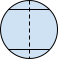
\includegraphics[width=0.3\linewidth]{../common/03_billiard_ai/resources/05_energy_transfer_node.png}
    \end{center}
\end{minipage}\hfill
\begin{minipage}[t]{0.8\textwidth}
    \textbf{Energy-Transfer-Node (Collision-Node)}: Dieser Node beschreibt die Übergabe von Energie auf die
    beteiligten Objekte.
\end{minipage}\vskip.2\baselineskip
Der Energy-Transfer-Node wird in drei Schichten aufgeteilt. Bei der Input-Schicht wird die Kantenfunktion (siehe S. \pageref{cust:Kantenfunktion})
angewendet. Diese berücksichtigt den Energieverlust bis zum Auftreten des Ereignisses. Die mittlere Schicht beschreibt
die Übergabefunktion der beteiligten Objekte. Die dritte Schicht repräsentiert das Resultat, also den Status der
Objekte nach der Energieübergabe.
\begin{figure}[h!]
    \begin{center}
        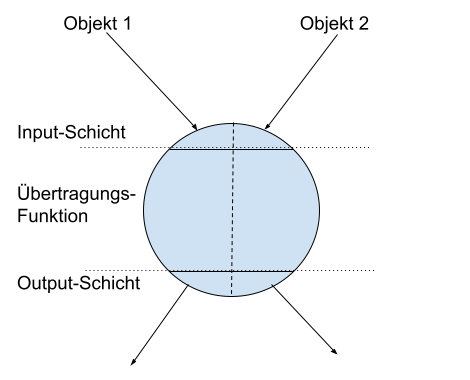
\includegraphics[width=0.5\linewidth]{../common/03_billiard_ai/resources/09_collision_node_description.png}
    \end{center}
    \caption{Der Energy-Transfer-Node}
    \label{fig:Der Energy-Transfer-Node}
\end{figure}\\
\begin{minipage}[t]{0.2\textwidth}
    \begin{center}
        
\includegraphics[width=0.3\linewidth]{../common/03_billiard_ai/resources/06_no_energy_node.png}
    \end{center}
\end{minipage}\hfill
\begin{minipage}[t]{0.8\textwidth}
    \textbf{No-Energy-Node}: Dieser Node wird eingesetzt, sobald der Energiewert eines variablen Objekts auf 0 sinkt und
    somit auch den Übergang von dynamisch zu statisch repräsentiert.
\end{minipage}\vskip.2\baselineskip
\begin{minipage}[t]{0.2\textwidth}
    \begin{center}
        
\includegraphics[width=0.3\linewidth]{../common/03_billiard_ai/resources/07_out_of_system_node.png}
    \end{center}
\end{minipage}\hfill
\begin{minipage}[t]{0.8\textwidth}
    \textbf{Out-Of-System-Node}: Dieser Node wird eingesetzt, sobald ein variables Objekt das System verlässt.
\end{minipage}\vskip.2\baselineskip
\begin{minipage}[t]{0.2\textwidth}
    \begin{center}
        
\includegraphics[width=0.3\linewidth]{../common/03_billiard_ai/resources/08_cutting_node.png}
    \end{center}
\end{minipage}\hfill
\begin{minipage}[t]{0.8\textwidth}
    \textbf{Cutting-Node}: Dieser Node ist ein spezieller Energy-Transfer-Node. Er wird bei variablen Objekten
    eingesetzt, die nicht an einem Ereignis beteiligt sind, wenn ein solches auftritt. Zum Ereigniszeitpunkt wird
    ein neuer Layer (siehe S. \pageref{cust:Layer}) geschaffen, welcher die Objekte, die am Ereignis beteiligt sind,
    in einem Energy-Transfer-Node festhält. Weiterhin wird der Status aller dynamsichen Objekte ebenfalls zu diesem
    Zeitpunkt festgehalten. Der Cutting-Node beschränkt sich auf ein Input- sowie Output-Objekt und beinhaltet als
    Energieübertragungsfunktion die Identitätsfunktion.
\end{minipage}\vskip.2\baselineskip

\subsection{Kantenfunktion} \label{cust:Kantenfunktion}
Die Kantenfunktion beschreibt eine Energieabnahme über die Zeit oder den Weg.

\subsection{Layer} \label{cust:Layer}
Sobald ein Ereignis auftritt wird ein neuer Layer im System eingefügt. Dieser beinhaltet sämtliche
Veränderungen der variablen Objekte und beschreibt den Status des Systems komplett. Der erste sowie der letzte Layer sind speziell, da diese eigentlich
nur deren Halbe sind. Ein Layer wird grundsätzlich in zwei Bereiche aufgeteilt. Es gibt den Inputbereich, welcher den
Status eines variablen Objektes vor der Energieübertragung, sowie den Outputbereich, welcher den Status
eines variablen Objektes nach der Energieübertragung beschreibt.
Um den aktuellen Stand eines Systems zu ermitteln, kann zwischen der Zeit des Outputbereichts von Layer $n-1$ wie der
Zeit des Inputbereichst von Layer $n$ interpoliert werden.

\subsection{Beispiel eines Graphen}
Das beschriebene Datenmodell kann als Graph\footnote{Aus effizientsgründen wird auf einen Graphen in der Implementation
verzichtet. Das System setzt sich aus verschiedenen Layern zusammen, bei welchen die Informationen der Events für jedes
variable Objekt separat und mit Zugriffszeit $O(1)$ abgelegt werden.} visualisiert werden. Als Beispiel wird die Idee
eines Billardstosses in Abbildung \ref{fig:Beispiel für ein Resultat des Algorithmus phys_sys} hinzugezogen.
Auf dem Tisch liegt eine weisse wie auch zwei rote Kugeln. Die zweite rote Kugel wird an keiner Interaktion beteiligt sein,
weswegen sie ihren Zustand nie verändert. Es ist ersichtlich, dass bei jedem Ereignis jeweils ein \glqq Out-of-energy-Node\grqq{}
eingefügt wird. Das erste Event beschreibt die Kollision des dynamischen Objekts \glqq weisse Kugel\grqq{} sowie des
statischen Objekts \glqq rote Kugel\grqq{}. Danach verliert die weisse Kugel sämtliche Energie und wechselt in den
Status \glqq{} Out-of-energy\grqq{}. Da die rote Kugel zu diesem Zeitpunkt dynamisch ist, wird für sie ein
\glqq{} Cutting-Node\grqq{} eingefügt. Zuletzt verlässt die rote Kugel das System, für sie wird ein \glqq{} Out-of-system-Node\grqq{}
erstellt und das System hat sämtliche Energie verloren. Ein Endzustand wurde erreicht. Es gilt weiterhin die Beschreibung
auf der linken Seite der Keyframes zu beachten. Ein Layer definiert immer deren zwei Keyframes, sofern es sich nicht um
den Input- oder Output-Layer handelt. Um den Zustand des Systems zu einem beliebigen Zeitpunkt zu berechnen, kann
jeweils zwischen den KeyFrames $n$ und $n + 1$ zweier Layer interpoliert werden.
\begin{figure}[h!]
    \begin{center}
        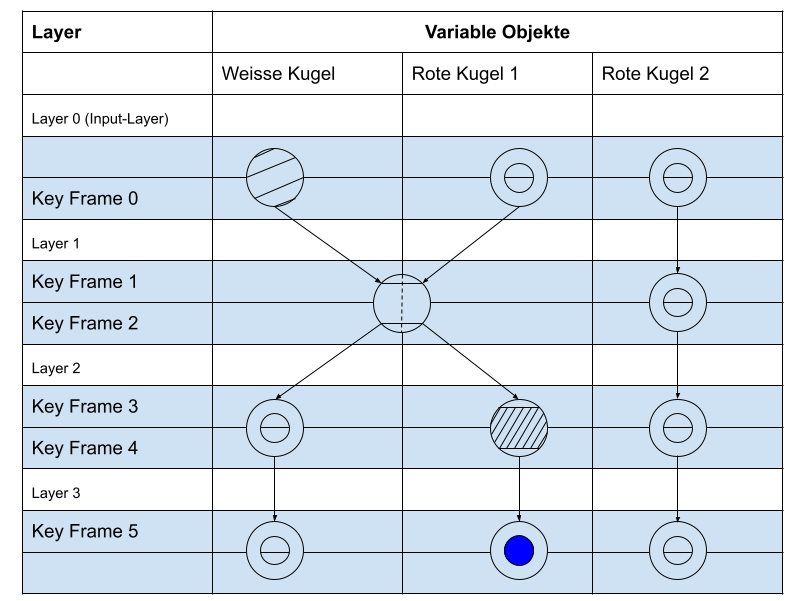
\includegraphics[width=0.6\linewidth]{../common/03_billiard_ai/resources/10_datenmodell_beispiel.png}
    \end{center}
    \caption{Beispiel für ein Resultat des Algorithmus \ref{alg:physikalisches_system}}
    \label{fig:Beispiel für ein Resultat des Algorithmus phys_sys}
\end{figure}

\begin{algorithm}[H]
    \DontPrintSemicolon
    \SetKwFunction{simulate}{simulate}
    \SetKwFunction{nextEvent}{nextEvent}
    \SetKwProg{Fn}{Function}{}{}
    \Fn{\simulate{start: Layer, constantObjects: list} $\longrightarrow$ System}{
        system $\longleftarrow$ System()\\
        system $\longleftarrow$ appendLayer(system, start)\\
        \While{! system.isStatic()}{
            nextEvent $\longleftarrow$ nextEvent(system.lastLayer(), constantObjects)\\
            layer $\longleftarrow$ atMoment(nextEvent)\\
            system $\longleftarrow$ appendLayer(system, start)
        }
        \KwRet system
    }
    \;
    \Fn{\nextEvent{layer: Layer, constantObjects: list} $\longrightarrow$ Node}{
        nextEvent: Node $\longleftarrow$ none\\
        \For{object in layer.dynamicObjects()}{
            nextEvent $\longleftarrow$ min(nextEvent, outOfEnergy(object))\\
            nextEvent $\longleftarrow$ min(nextEvent, collision(object, layer.dynamicObjects()))\\
            nextEvent $\longleftarrow$ min(nextEvent, collision(object, layer.staticObjects()))\\
            nextEvent $\longleftarrow$ min(nextEvent, collision(object, constantObjects))
        }
        \KwRet nextEvent
    }
    \caption{Algorithmus zum Aufbau eines physikalischen Systems}
    \label{alg:physikalisches_system}
\end{algorithm}
In Algorithmus \ref{alg:physikalisches_system} wird die Grundidee erläutert. Als Input für die Funktion \glqq simulate\grqq{}
dient der erste Layer, welcher mehrere variable Objekte beinhalten kann, wobei mindestens ein Objekt dynamisch (energiereich)
sein sollte. Dieser Layer wird direkt dem erzeugten System hinzugefügt und dieses wird solange bearbeitet, bis alle variablen
Objekte statisch sind (das System hat keine Energie mehr). In jedem Schleifendurchlauf wird das nächste Event berechnet.
Die Events können diverser Natur sein. Es werden Kollisionen mit dynamischen, statischen wie auch konstanten Objekten
geprüft. Bei der Kollision mit konstanten Objekten können die Ereignisse \glqq Energy transfer\grqq{} oder \glqq Out of
System\grqq{} auftreten. Weiterhin wird geprüft, ob ein dynamisches Objekt seine Energie durch die Kantenfunktion
verliert. Auf Basis dieses Events wird dann ein neuer Layer generiert, welcher für die am Event beteiligten Objekte
den entsprechenden Node einfügen und für die anderen variablen Objekte entweder ein \glqq Cutting-Node\grqq{} oder ein
\glqq{} Out-of-energy-Node\grqq{} berechnet wird.